\documentclass[11pt,a4paper]{report}
\usepackage[textwidth=37em,vmargin=30mm]{geometry}
\usepackage{calc,xunicode,amsmath,amssymb,paralist,enumitem,tabu,booktabs,datetime2,xeCJK,xeCJKfntef,listings}
\usepackage{tocloft,fancyhdr,tcolorbox,xcolor,graphicx,eso-pic,xltxtra,xelatexemoji}

\newcommand{\envyear}[0]{2025}
\newcommand{\envdatestr}[0]{2025-01-19}
\newcommand{\envfinaldir}[0]{webdb/2025/20250119/final}

\usepackage[hidelinks]{hyperref}
\hypersetup{
    colorlinks=false,
    pdfpagemode=FullScreen,
    pdftitle={Web Digest - \envdatestr}
}

\setlength{\cftbeforechapskip}{10pt}
\renewcommand{\cftchapfont}{\rmfamily\bfseries\large\raggedright}
\setlength{\cftbeforesecskip}{2pt}
\renewcommand{\cftsecfont}{\sffamily\small\raggedright}

\setdefaultleftmargin{2em}{2em}{1em}{1em}{1em}{1em}

\usepackage{xeCJK,xeCJKfntef}
\xeCJKsetup{PunctStyle=plain,RubberPunctSkip=false,CJKglue=\strut\hskip 0pt plus 0.1em minus 0.05em,CJKecglue=\strut\hskip 0.22em plus 0.2em}
\XeTeXlinebreaklocale "zh"
\XeTeXlinebreakskip = 0pt


\setmainfont{Brygada 1918}
\setromanfont{Brygada 1918}
\setsansfont{IBM Plex Sans}
\setmonofont{JetBrains Mono NL}
\setCJKmainfont{Noto Serif CJK SC}
\setCJKromanfont{Noto Serif CJK SC}
\setCJKsansfont{Noto Sans CJK SC}
\setCJKmonofont{Noto Sans CJK SC}

\setlength{\parindent}{0pt}
\setlength{\parskip}{8pt}
\linespread{1.15}

\lstset{
	basicstyle=\ttfamily\footnotesize,
	numbersep=5pt,
	backgroundcolor=\color{black!5},
	showspaces=false,
	showstringspaces=false,
	showtabs=false,
	tabsize=2,
	captionpos=b,
	breaklines=true,
	breakatwhitespace=true,
	breakautoindent=true,
	linewidth=\textwidth
}






\newcommand{\coverpic}[2]{
    % argv: itemurl, authorname
    Cover photo by #2~~(\href{#1}{#1})
}
\newcommand{\makeheader}[0]{
    \begin{titlepage}
        % \newgeometry{hmargin=15mm,tmargin=21mm,bmargin=12mm}
        \begin{center}
            
            \rmfamily\scshape
            \fontspec{BaskervilleF}
            \fontspec{Old Standard}
            \fontsize{59pt}{70pt}\selectfont
            WEB\hfill DIGEST
            
            \vfill
            % \vskip 30pt
            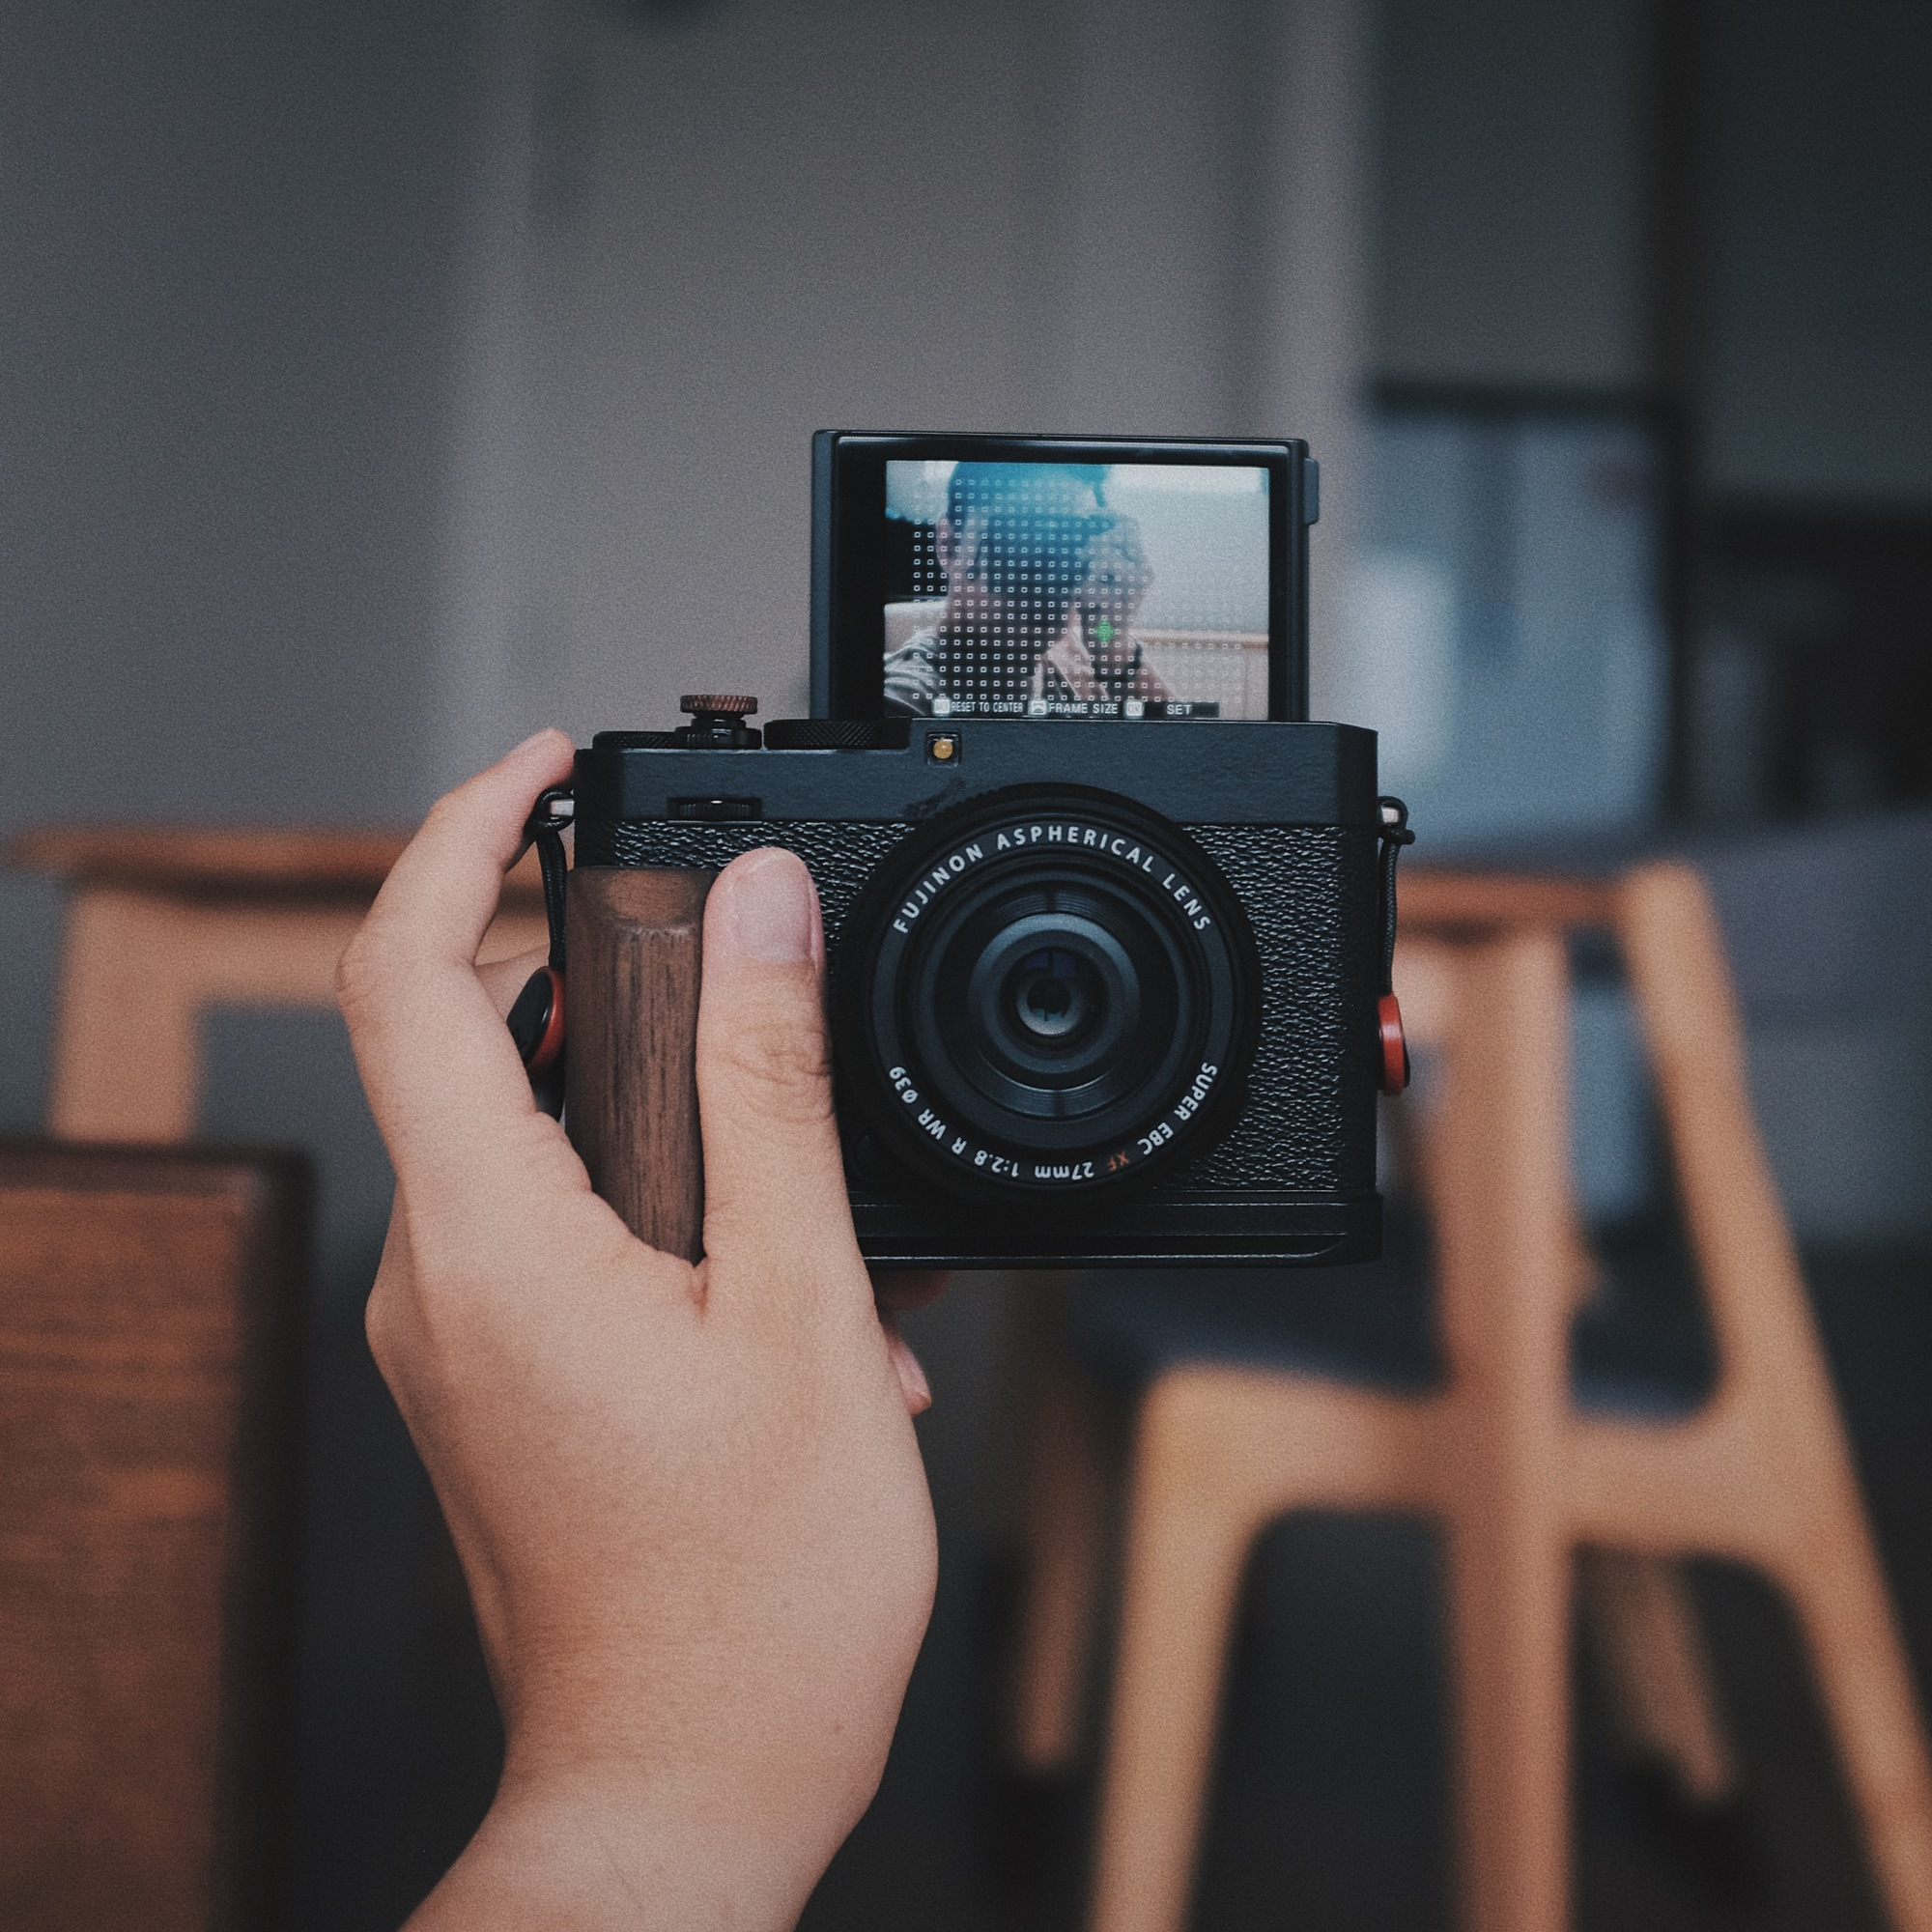
\includegraphics[width=\linewidth]{\envfinaldir/coverpic-prod.jpg}\par
            % \vskip 30pt
            \vfill

            \normalsize\rmfamily\scshape
            \copyright{} The Web Digest Project \hfill\large \envdatestr
        \end{center}
    \end{titlepage}
    % \restoregeometry
}
\newcommand{\simplehref}[1]{%
    \textcolor{blue!80!green}{\href{#1}{#1}}%
}
\renewcommand{\contentsname}{\center\Huge\sffamily\bfseries Contents\par\vskip 20pt}
\newcounter{ipartcounter}
\setcounter{ipartcounter}{0}
\newcommand{\ipart}[1]{
    % \vskip 20pt
    \clearpage
    \stepcounter{ipartcounter}
    \phantomsection
    \addcontentsline{toc}{chapter}{#1}
    % \begin{center}
    %     \Huge
    %     \sffamily\bfseries
    %     #1
    % \end{center}
    % \vskip 20pt plus 7pt
}
\newcounter{ichaptercounter}
\setcounter{ichaptercounter}{0}
\newcommand{\ichapter}[1]{
    % \vskip 20pt
    \clearpage
    \stepcounter{ichaptercounter}
    \phantomsection
    \addcontentsline{toc}{section}{\numberline{\arabic{ichaptercounter}}#1}
    \begin{center}
        \Huge
        \sffamily\bfseries
        #1
    \end{center}
    \vskip 20pt plus 7pt
}
\newcommand{\entrytitlefont}[1]{\subsection*{\raggedright\Large\sffamily\bfseries#1}}
\newcommand{\entryitemGeneric}[2]{
    % argv: title, url
    \parbox{\linewidth}{
        \entrytitlefont{#1}\par\vskip 5pt
        \footnotesize\ttfamily\mdseries
        \simplehref{#2}
    }\vskip 11pt plus 11pt minus 1pt
}
\newcommand{\entryitemGithub}[3]{
    % argv: title, url, desc
    \parbox{\linewidth}{
        \entrytitlefont{#1}\par\vskip 5pt
        \footnotesize\ttfamily\mdseries
        \simplehref{#2}\par\vskip 5pt
        \small\rmfamily\mdseries#3
    }\vskip 11pt plus 11pt minus 1pt
}
\newcommand{\entryitemAp}[3]{
    % argv: title, url, desc
    \parbox{\linewidth}{
        \entrytitlefont{#1}\par\vskip 5pt
        \footnotesize\ttfamily\mdseries
        \simplehref{#2}\par\vskip 5pt
        \small\rmfamily\mdseries#3
    }\vskip 11pt plus 11pt minus 1pt
}
\newcommand{\entryitemHackernews}[3]{
    % argv: title, hnurl, rawurl
    % \parbox{\linewidth}{
    %     \entrytitlefont{#1}\par\vskip 5pt
    %     \footnotesize\ttfamily\mdseries
    %     \simplehref{#3}\par
    %     \textcolor{black!50}{\href{#2}{#2}}
    % }\vskip 11pt plus 11pt minus 1pt
    \begin{minipage}{\linewidth}
            \entrytitlefont{#1}\par\vskip 5pt
            \footnotesize\ttfamily\mdseries
            \simplehref{#3}\par
            \textcolor{black!50}{\href{#2}{#2}}
    \end{minipage}\par\vskip 11pt plus 11pt minus 1pt
}







\begin{document}

\makeheader

\tableofcontents\clearpage




\ipart{Developers}
\ichapter{Hacker News}
\entryitemTwoLinks{Amazon's AI crawler is making my Git server unstable}{https://news.ycombinator.com/item?id=42750420}{https://xeiaso.net/notes/2025/amazon-crawler/}

\entryitemTwoLinks{VS Code Pets}{https://news.ycombinator.com/item?id=42750195}{https://github.com/tonybaloney/vscode-pets}

\entryitemTwoLinks{O1 isn't a chat model (and that's the point)}{https://news.ycombinator.com/item?id=42750096}{https://www.latent.space/p/o1-skill-issue}

\entryitemTwoLinks{Show HN: Interactive systemd – a better way to work with systemd units}{https://news.ycombinator.com/item?id=42749402}{https://isd-project.github.io/isd/}

\entryitemTwoLinks{Dusa Programming Language (Finite-Choice Logic Programming)}{https://news.ycombinator.com/item?id=42749147}{https://dusa.rocks/docs/}

\entryitemTwoLinks{Why do bees die when they sting you?}{https://news.ycombinator.com/item?id=42749069}{https://www.subanima.org/bees/}

\entryitemTwoLinks{Ask HN: Has anyone tried alternative company models (like a co-op) for SaaS?}{https://news.ycombinator.com/item?id=42748394}{https://news.ycombinator.com/item?id=42748394}

\entryitemTwoLinks{The Toyota Prius transformed the auto industry}{https://news.ycombinator.com/item?id=42747899}{https://spectrum.ieee.org/toyota-prius-transformed-auto-industry}

\entryitemTwoLinks{Windows BitLocker – Screwed Without a Screwdriver}{https://news.ycombinator.com/item?id=42747877}{https://neodyme.io/en/blog/bitlocker\_screwed\_without\_a\_screwdriver/}

\entryitemTwoLinks{The AMD Radeon Instinct MI300A's Giant Memory Subsystem}{https://news.ycombinator.com/item?id=42747864}{https://chipsandcheese.com/p/inside-the-amd-radeon-instinct-mi300as}

\entryitemTwoLinks{Google begins requiring JavaScript for Google Search}{https://news.ycombinator.com/item?id=42747092}{https://techcrunch.com/2025/01/17/google-begins-requiring-javascript-for-google-search/}

\entryitemTwoLinks{Honest Ahmed (2011)}{https://news.ycombinator.com/item?id=42747065}{https://bugzilla.mozilla.org/show\_bug.cgi?id=647959}

\entryitemTwoLinks{I've been advocating for RSS support, and you should too}{https://news.ycombinator.com/item?id=42746222}{https://reedybear.bearblog.dev/ive-been-advocating-for-rss-support-and-you-should-too/}

\entryitemTwoLinks{Using ChatGPT is not bad for the environment}{https://news.ycombinator.com/item?id=42745847}{https://andymasley.substack.com/p/individual-ai-use-is-not-bad-for}

\entryitemTwoLinks{Can you read this cursive handwriting? The National Archives wants your help}{https://news.ycombinator.com/item?id=42745334}{https://www.smithsonianmag.com/smart-news/can-you-read-this-cursive-handwriting-the-national-archives-wants-your-help-180985833/}

\entryitemTwoLinks{EFF statement on U.S. Supreme Court's decision to uphold TikTok ban}{https://news.ycombinator.com/item?id=42744695}{https://www.eff.org/deeplinks/2025/01/eff-statement-us-supreme-courts-decision-uphold-tiktok-ban}

\entryitemTwoLinks{Investigating an ``evil'' RJ45 dongle}{https://news.ycombinator.com/item?id=42743033}{https://lcamtuf.substack.com/p/investigating-an-evil-rj45-dongle}

\entryitemTwoLinks{So you want to build your own data center}{https://news.ycombinator.com/item?id=42743019}{https://blog.railway.com/p/data-center-build-part-one}

\entryitemTwoLinks{Show HN: Compile C to Not Gates}{https://news.ycombinator.com/item?id=42742350}{https://github.com/tomhea/c2fj}

\entryitemTwoLinks{Branchless UTF-8 Encoding}{https://news.ycombinator.com/item?id=42742184}{https://cceckman.com/writing/branchless-utf8-encoding/}\ichapter{Phoronix}
\entryitemGeneric{\hskip 0pt{}New "mountinfo" Program Set To Be Bundled With Linux 6.14}{https://www.phoronix.com/news/Linux-6.14-mountinfo}

\entryitemGeneric{\hskip 0pt{}QH Electronics Game Controller Support Being Added For Linux 6.14}{https://www.phoronix.com/news/QH-Electronics-XPad-Linux-6.14}

\entryitemGeneric{\hskip 0pt{}Linux 6.14 To Perform Better With The Drgn Debugger Via Faster /proc/kcore Reads}{https://www.phoronix.com/news/Linux-6.14-Faster-kcore-Reads}

\entryitemGeneric{\hskip 0pt{}GNU Debugger GDB 16.1 Brings Better Intel PT Support, gstack Added}{https://www.phoronix.com/news/GNU-Debugger-GDB-16.1}

\entryitemGeneric{\hskip 0pt{}Intel Tofino P4 Software Open-Sourced Years Later}{https://www.phoronix.com/news/Intel-Tofino-P4-Open-Source}

\entryitemGeneric{\hskip 0pt{}GNOME Snapshot Can Now Read QR Codes, Flatpak 1.16 Brings More Features}{https://www.phoronix.com/news/GNOME-48-Alpha-Week}

\entryitemGeneric{\hskip 0pt{}Year Of The BSD Desktop? There's Going To Be A BSD Desktop Conference At Least}{https://www.phoronix.com/news/BSD-Desktop-Conference-GhostBSD}

\entryitemGeneric{\hskip 0pt{}KDE Developers Fixing "Record Amounts Of Bugs" Following Plasma 6.3 Beta}{https://www.phoronix.com/news/KDE-Plasma-6.3-Bug-Fixing}

\entryitemGeneric{\hskip 0pt{}Wine 10.0-rc6 Released With Another 18 Bugs Fixed}{https://www.phoronix.com/news/Wine-10.0-rc6-Released}\ichapter{Dribbble}
\entryitemGeneric{\hskip 0pt{}Wine Label}{https://dribbble.com/shots/25490604-Wine-Label}

\entryitemGeneric{\hskip 0pt{}planet}{https://dribbble.com/shots/25490310-planet}

\entryitemGeneric{\hskip 0pt{}Shihiko // E-commerce Website}{https://dribbble.com/shots/25489208-Shihiko-E-commerce-Website}

\entryitemGeneric{\hskip 0pt{}Wine Label}{https://dribbble.com/shots/25485370-Wine-Label}

\entryitemGeneric{\hskip 0pt{}EA System Ambigram}{https://dribbble.com/shots/25486215-EA-System-Ambigram}

\entryitemGeneric{\hskip 0pt{}Puzzle Fintech Website Design}{https://dribbble.com/shots/25394559-Puzzle-Fintech-Website-Design}

\entryitemGeneric{\hskip 0pt{}RoundRobin 2.0}{https://dribbble.com/shots/25479558-RoundRobin-2-0}

\entryitemGeneric{\hskip 0pt{}Pemberton's Formula}{https://dribbble.com/shots/25480158-Pemberton-s-Formula}

\entryitemGeneric{\hskip 0pt{}Black Cats}{https://dribbble.com/shots/25478711-Black-Cats}

\entryitemGeneric{\hskip 0pt{}N\&R Social Media}{https://dribbble.com/shots/25159226-N-R-Social-Media}

\entryitemGeneric{\hskip 0pt{}Vertical Logos from the Portfolio}{https://dribbble.com/shots/25479968-Vertical-Logos-from-the-Portfolio}

\entryitemGeneric{\hskip 0pt{}Developing new skills}{https://dribbble.com/shots/25479409-Developing-new-skills}

\entryitemGeneric{\hskip 0pt{}Top 9 logos of 2024}{https://dribbble.com/shots/25479840-Top-9-logos-of-2024}

\entryitemGeneric{\hskip 0pt{}NEON Graphic Style}{https://dribbble.com/shots/25480590-NEON-Graphic-Style}

\entryitemGeneric{\hskip 0pt{}Gillespie Farms™}{https://dribbble.com/shots/25474556-Gillespie-Farms}

\entryitemGeneric{\hskip 0pt{}Document Scanner App}{https://dribbble.com/shots/25466972-Document-Scanner-App}

\entryitemGeneric{\hskip 0pt{}Faith Education Icons}{https://dribbble.com/shots/25422138-Faith-Education-Icons}

\entryitemGeneric{\hskip 0pt{}Round Robin}{https://dribbble.com/shots/25467606-Round-Robin}

\entryitemGeneric{\hskip 0pt{}Nexos crypto wallet}{https://dribbble.com/shots/25464532-Nexos-crypto-wallet}

\entryitemGeneric{\hskip 0pt{}Kraken Illustration}{https://dribbble.com/shots/25468020-Kraken-Illustration}

\entryitemGeneric{\hskip 0pt{}Glyph Beer 62}{https://dribbble.com/shots/25470954-Glyph-Beer-62}

\entryitemGeneric{\hskip 0pt{}B}{https://dribbble.com/shots/25466481-B}

\entryitemGeneric{\hskip 0pt{}The best route to the corner office}{https://dribbble.com/shots/25468475-The-best-route-to-the-corner-office}

\entryitemGeneric{\hskip 0pt{}Crypto Trading Website}{https://dribbble.com/shots/25463542-Crypto-Trading-Website}


\ipart{Developers~~~~(zh-Hans)}
\ichapter{Solidot}
\entryitemGeneric{\hskip 0pt{}原神被禁止向美国 16 岁以下儿童出售战利品箱}{https://www.solidot.org/story?sid=80367}

\entryitemGeneric{\hskip 0pt{}CNNIC 报告称中国有 2.49 亿人使用过生成式 AI}{https://www.solidot.org/story?sid=80366}

\entryitemGeneric{\hskip 0pt{}TikTok 在美最高法院败诉,准备周日关闭美国服务}{https://www.solidot.org/story?sid=80365}

\entryitemGeneric{\hskip 0pt{}科学家发现爱阅读的人的大脑与不爱阅读的人有差别}{https://www.solidot.org/story?sid=80364}

\entryitemGeneric{\hskip 0pt{}南方古猿的肉食量不大}{https://www.solidot.org/story?sid=80363}

\entryitemGeneric{\hskip 0pt{}考古学家在英国发现一个铁器时代的母系社会}{https://www.solidot.org/story?sid=80362}

\entryitemGeneric{\hskip 0pt{}Meta 朝通用翻译器前进了一大步}{https://www.solidot.org/story?sid=80361}

\entryitemGeneric{\hskip 0pt{}中国核电发电量到 2030 年将超越欧美}{https://www.solidot.org/story?sid=80360}

\entryitemGeneric{\hskip 0pt{}1984 年版《沙丘》导演大卫林奇去世}{https://www.solidot.org/story?sid=80359}

\entryitemGeneric{\hskip 0pt{}任天堂首席法务承认模拟器本身是合法的}{https://www.solidot.org/story?sid=80358}

\entryitemGeneric{\hskip 0pt{}小红书据报道可能切割中国用户和外国用户}{https://www.solidot.org/story?sid=80357}

\entryitemGeneric{\hskip 0pt{}任天堂正式宣布 Switch 2}{https://www.solidot.org/story?sid=80356}

\entryitemGeneric{\hskip 0pt{}科学家在深度学习帮助下设计出全新的中和蛇毒的蛋白质}{https://www.solidot.org/story?sid=80355}

\entryitemGeneric{\hskip 0pt{}碳元素如何在宇宙中扩散?}{https://www.solidot.org/story?sid=80354}

\entryitemGeneric{\hskip 0pt{}RISC-V 开发商算能公司被美国列入实体名单}{https://www.solidot.org/story?sid=80353}

\entryitemGeneric{\hskip 0pt{}Blue Origin 的重型火箭 New Glenn 首次抵达轨道}{https://www.solidot.org/story?sid=80352}

\entryitemGeneric{\hskip 0pt{}Proton CEO 拥抱特朗普引发争议}{https://www.solidot.org/story?sid=80351}

\entryitemGeneric{\hskip 0pt{}动视对微软 Xbox Game Pass 订阅量增加帮助不大}{https://www.solidot.org/story?sid=80350}

\entryitemGeneric{\hskip 0pt{}日英意下一代战斗机计划本年内开始制造试制机}{https://www.solidot.org/story?sid=80349}

\entryitemGeneric{\hskip 0pt{}新泽西州州长呼吁 K-12 学校禁止学生使用手机}{https://www.solidot.org/story?sid=80348}\ichapter{V2EX}
\entryitemGeneric{\hskip 0pt{}[问与答] 帮朋友问,公司需要建立一个 AI 算力中心,提供算力给其他公司使用,请问如何搭建?}{https://www.v2ex.com/t/1106178}

\entryitemGeneric{\hskip 0pt{}[iCloud] 请问 icloud 拼车哪里靠谱啊}{https://www.v2ex.com/t/1106177}

\entryitemGeneric{\hskip 0pt{}[分享发现] 难道 Steam 的账户密码是明文储存的??}{https://www.v2ex.com/t/1106176}

\entryitemGeneric{\hskip 0pt{}[分享发现] 紫藤巷杀人案离奇内情:四个专案组与警界``内鬼''  紫藤巷杀人案离奇内情:四个专案组与警界``内鬼''  紫藤巷杀人案离奇内情:四个专案组与警界``内鬼''}{https://www.v2ex.com/t/1106175}

\entryitemGeneric{\hskip 0pt{}[问与答] 关于 vidhub、infuse 的一些疑问}{https://www.v2ex.com/t/1106174}

\entryitemGeneric{\hskip 0pt{}[Android] 国补换机,求推荐安卓手机}{https://www.v2ex.com/t/1106173}

\entryitemGeneric{\hskip 0pt{}[程序员] aiofferly 刷题}{https://www.v2ex.com/t/1106172}

\entryitemGeneric{\hskip 0pt{}[问与答] 现在真的是 All in AI}{https://www.v2ex.com/t/1106171}

\entryitemGeneric{\hskip 0pt{}[问与答] 摸鱼大佬们,求个 CPE/随身 Wifi 选购体验/建议/指南。}{https://www.v2ex.com/t/1106170}

\entryitemGeneric{\hskip 0pt{}[Python] py 的异步队列选择 celery arq drm rq ,好像还有一个国人大佬写的(忘了叫啥?名字貌似起的很直白,很牛逼。)}{https://www.v2ex.com/t/1106168}

\entryitemGeneric{\hskip 0pt{}[推广] (VPS)Zgo 优质落地解锁机 线路机及高性能 VDS}{https://www.v2ex.com/t/1106167}

\entryitemGeneric{\hskip 0pt{}[Android] android 版本的 youtube 上傳視頻長度小於 3 分鐘會自動發布成短視頻而不是長視頻咋解決?}{https://www.v2ex.com/t/1106164}

\entryitemGeneric{\hskip 0pt{}[分享发现] 选择 SSLManage,开启自动化证书管理之旅}{https://www.v2ex.com/t/1106163}

\entryitemGeneric{\hskip 0pt{}[程序员] 2025 年有哪些值得去技术大会呀}{https://www.v2ex.com/t/1106162}

\entryitemGeneric{\hskip 0pt{}[问与答] 买了荣耀 GT PRO 平板,求推荐平替好用的手写笔}{https://www.v2ex.com/t/1106161}

\entryitemGeneric{\hskip 0pt{}[问与答] 为父母购买了商业医保后,如何能让他们在家自行操作理赔}{https://www.v2ex.com/t/1106160}

\entryitemGeneric{\hskip 0pt{}[求职] 25 届秋招惨败,怎么全是实习!}{https://www.v2ex.com/t/1106159}

\entryitemGeneric{\hskip 0pt{}[分享发现] 经典版 QQ 里的 800GB 聊天记录大概是废了}{https://www.v2ex.com/t/1106158}

\entryitemGeneric{\hskip 0pt{}[职场话题] 今天公司聚餐,喝了几杯红酒,现在感觉很后悔,以后再也不喝了}{https://www.v2ex.com/t/1106157}

\entryitemGeneric{\hskip 0pt{}[iOS] 关于在 iPad 和 Mac 上运行某些 iOS 应用的返回操作}{https://www.v2ex.com/t/1106156}

\entryitemGeneric{\hskip 0pt{}[NAS] 求助:如何实现 NAS 数据的远程备份(百度云)}{https://www.v2ex.com/t/1106155}

\entryitemGeneric{\hskip 0pt{}[Apple] 一年多的 MBP,电池循环才 50 出头,健康度就 89\%了,这么离谱的吗}{https://www.v2ex.com/t/1106154}

\entryitemGeneric{\hskip 0pt{}[职场话题] 长安真的是没法呆了,年前又来一波}{https://www.v2ex.com/t/1106153}

\entryitemGeneric{\hskip 0pt{}[程序员] 从微服务走向单体化}{https://www.v2ex.com/t/1106152}

\entryitemGeneric{\hskip 0pt{}[宽带症候群] 晚上 B 站网页一直转圈}{https://www.v2ex.com/t/1106151}

\entryitemGeneric{\hskip 0pt{}[macOS] macOS 的时间机器硬盘怎么选好?}{https://www.v2ex.com/t/1106148}

\entryitemGeneric{\hskip 0pt{}[生活] 今天被老妈的询问搞得突然第一次不想回家}{https://www.v2ex.com/t/1106147}

\entryitemGeneric{\hskip 0pt{}[分享创造] 在用 ai 编程工具的可以看一下}{https://www.v2ex.com/t/1106144}

\entryitemGeneric{\hskip 0pt{}[分享创造] V2EX 抽奖小程序}{https://www.v2ex.com/t/1106143}

\entryitemGeneric{\hskip 0pt{}[Android] Root 真的还是刚需吗}{https://www.v2ex.com/t/1106142}

\entryitemGeneric{\hskip 0pt{}[iPhone] iPhone 16 pro max 相机开机黑屏}{https://www.v2ex.com/t/1106140}

\entryitemGeneric{\hskip 0pt{}[问与答] 澳洲转运国内哪家转运公司靠谱}{https://www.v2ex.com/t/1106139}

\entryitemGeneric{\hskip 0pt{}[分享发现] 最强 follow 源(第 2 期:最强小涩站)}{https://www.v2ex.com/t/1106138}

\entryitemGeneric{\hskip 0pt{}[全球工单系统] misakaf 疑似跑路了?}{https://www.v2ex.com/t/1106134}

\entryitemGeneric{\hskip 0pt{}[问与答] 不需要手机号能用的邮箱?}{https://www.v2ex.com/t/1106133}

\entryitemGeneric{\hskip 0pt{}[问与答] 使用阿里云盘的看过来}{https://www.v2ex.com/t/1106131}

\entryitemGeneric{\hskip 0pt{}[问与答] RouterOS UDP 端口转发无法保留源 IP}{https://www.v2ex.com/t/1106130}

\entryitemGeneric{\hskip 0pt{}[问与答] 我的服务器被 DDOS 攻击了,恶人他图啥?}{https://www.v2ex.com/t/1106129}

\entryitemGeneric{\hskip 0pt{}[分享创造] 女朋友给我做了一个小游戏(~ ̄▽ ̄)~}{https://www.v2ex.com/t/1106128}

\entryitemGeneric{\hskip 0pt{}[程序员] 尴尬了,为租机老板做了个 工具,差不多好了,他不要了!😭}{https://www.v2ex.com/t/1106127}

\entryitemGeneric{\hskip 0pt{}[程序员] 都有什么站长工具,能提交到爬虫的之类的网站?}{https://www.v2ex.com/t/1106126}

\entryitemGeneric{\hskip 0pt{}[问与答] Obsidian self-hosted livesync 使用求助}{https://www.v2ex.com/t/1106125}

\entryitemGeneric{\hskip 0pt{}[问与答] 农村家用室外摄像头推荐}{https://www.v2ex.com/t/1106124}

\entryitemGeneric{\hskip 0pt{}[问与答] 孕 6 周需要检查哪些项目?}{https://www.v2ex.com/t/1106123}

\entryitemGeneric{\hskip 0pt{}[生活] 两轮电动自行车推荐}{https://www.v2ex.com/t/1106122}

\entryitemGeneric{\hskip 0pt{}[问与答] 有哪些事情是你觉得``人教人教不会,事教人一教就会''的?}{https://www.v2ex.com/t/1106121}

\entryitemGeneric{\hskip 0pt{}[小米] 请问:小米运动是否有年度总结能力或工具}{https://www.v2ex.com/t/1106119}

\entryitemGeneric{\hskip 0pt{}[分享创造] 分享便民服务的网站}{https://www.v2ex.com/t/1106118}

\entryitemGeneric{\hskip 0pt{}[问与答] 你们有没有发现最近百度盘速度快了}{https://www.v2ex.com/t/1106117}

\entryitemGeneric{\hskip 0pt{}[程序员] 服了,天天都有 cursor 的帖子}{https://www.v2ex.com/t/1106116}


\ipart{Generic News}
\ichapter{Reuters}
\entryitemWithDescription{\hskip 0pt{}South Korean court extends President Yoon's detention}{https://www.reuters.com/world/asia-pacific/south-korean-court-grants-extension-president-yoons-detention-2025-01-18/}{A South Korean court granted on Sunday an extension of President Yoon Suk Yeol\textquotesingle s detention, saying there was "concern" that Yoon could "destroy evidence" in a criminal probe related to his short-lived declaration of...}

\entryitemWithDescription{\hskip 0pt{}Canada cabinet minister Gould says she is running to replace Trudeau}{https://www.reuters.com/world/americas/canada-cabinet-minister-gould-says-she-is-running-replace-trudeau-2025-01-18/}{Canadian cabinet minister Karina Gould on Saturday said she would take part in the contest to replace Prime Minister Justin Trudeau as leader of the ruling Liberal...}

\entryitemWithDescription{\hskip 0pt{}Trump immigration forces to target multiple cities, border czar says}{https://www.reuters.com/world/us/trump-immigration-forces-target-multiple-cities-border-czar-says-2025-01-18/}{President-elect Donald Trump\textquotesingle s incoming "border czar" Tom Homan said on Saturday that targeted operations to detain migrants who are in the U.S. illegally will begin next week, and indicated they would involve several...}

\entryitemWithDescription{\hskip 0pt{}Trump's return to Washington before inauguration features fireworks, Elvis impersonator}{https://www.reuters.com/world/us/trumps-return-washington-before-inauguration-features-fireworks-elvis-2025-01-18/}{President-elect Donald Trump is set to arrive in Washington on Saturday evening for an inauguration celebration marking his return to power that has been upended by record cold...}

\entryitemWithDescription{\hskip 0pt{}Last-gasp Nunez double gives Liverpool 2-0 win at Brentford}{https://www.reuters.com/sports/soccer/last-gasp-nunez-double-gives-liverpool-2-0-win-brentford-2025-01-18/}{Substitute Darwin Nunez\textquotesingle s stoppage-time double gave Liverpool a 2-0 win at Brentford on Saturday, as the Premier League leaders left it late to record their first league win of...}

\entryitemWithDescription{\hskip 0pt{}Thousands gather in Washington to protest Trump inauguration}{https://www.reuters.com/world/us/thousands-gather-washington-protest-trump-inauguration-2025-01-18/}{Demonstrators rallied for abortion and immigration rights as well as local D.C...}

\entryitemWithDescription{\hskip 0pt{}Austin Tice's mother, in Damascus, hopes to find son missing since 2012}{https://www.reuters.com/world/austin-tices-mother-damascus-hopes-find-son-missing-since-2012-2025-01-18/}{The mother of American journalist Austin Tice, who was taken captive during a reporting trip to Syria in August 2012, arrived in Damascus on Saturday to step up the search for her son and said she hopes she can take him home with...}

\entryitemWithDescription{\hskip 0pt{}Russia says it will counter any UK-Ukraine cooperation in Sea of Azov}{https://www.reuters.com/world/europe/russia-says-it-will-counter-any-uk-ukraine-cooperation-sea-azov-2025-01-18/}{The Russian Foreign Ministry said on Saturday Ukraine and Britain "had no room" for cooperation in the Sea of Azov, commenting on a new 100-year partnership agreement between Kyiv and London the two countries\textquotesingle{} leaders...}

\entryitemWithDescription{\hskip 0pt{}Fuel tanker truck blast kills at least 60 in Nigeria}{https://www.reuters.com/world/africa/fuel-tanker-truck-explosion-kills-least-60-people-nigeria-2025-01-18/}{At least 60 people were killed and more injured in northern Nigeria on Saturday when a petrol tanker truck overturned, spilling fuel that exploded, the Federal Road Safety Corps (FRSC...}

\entryitemWithDescription{\hskip 0pt{}Power outages hit army-controlled Sudan after drone attacks}{https://www.reuters.com/world/africa/blackouts-hit-wide-swathes-army-controlled-sudan-after-drone-attacks-2025-01-18/}{Areas impacted by the cuts are housing millions of internally displaced people, straining living space and...}

\entryitemWithDescription{\hskip 0pt{}India police detain second suspect in Saif Ali Khan stabbing incident}{https://www.reuters.com/world/india/india-police-detain-second-suspect-saif-ali-khan-stabbing-incident-2025-01-18/}{Police in the central Indian state of Chhattisgarh on Saturday detained a second person suspected of involvement in a knife attack in which Bollywood actor Saif Ali Khan was...}

\entryitemWithDescription{\hskip 0pt{}Dozens injured, trapped in a ski lift accident in northern Spain}{https://www.reuters.com/world/europe/dozens-injured-trapped-ski-lift-accident-north-spain-2025-01-18/}{Around 80 people remain trapped, hanging in the chairlift at the ski resort of Astún, in the province of Huesca, state TV channel TVE...}

\entryitemWithDescription{\hskip 0pt{}Trump says he may give TikTok a 90-day reprieve Monday}{https://www.reuters.com/technology/tiktok-faces-us-ban-deadline-users-brace-fallout-2025-01-18/}{Users on the app were saying their goodbyes, some filming themselves frantically scrolling or sharing final secrets with their followers ahead of the possible...}






\clearpage
\leavevmode\vfill
\footnotesize

Copyright \copyright{} 2023-2025 Neruthes and other contributors.

This document is published with CC BY-NC-ND 4.0 license.

The entries listed in this newsletter may be copyrighted by their respective creators.

This newsletter is generated by the Web Digest project.

The newsletters are also delivered via Telegram channel \CJKunderline{\href{https://t.me/webdigestchannel}{https://t.me/webdigestchannel}}.\\
RSS feed is available at \CJKunderline{\href{https://webdigest.pages.dev/rss.xml}{https://webdigest.pages.dev/rss.xml}}.

This newsletter is available in PDF at
\CJKunderline{\href{https://webdigest.pages.dev/}{https://webdigest.pages.dev/}}.

The source code being used to generate this newsletter is available at\\
\CJKunderline{\href{https://github.com/neruthes/webdigest}{https://github.com/neruthes/webdigest}}.

This newsletter is also available in
\CJKunderline{\href{http://webdigest.pages.dev/readhtml/\envyear/WebDigest-20250119.html}{HTML}} and
\CJKunderline{\href{https://github.com/neruthes/webdigest/blob/master/markdown/\envyear/WebDigest-20250119.md}{Markdown}}.


\coverpic{https://unsplash.com/photos/a-view-of-a-mountain-covered-in-fog-hfvaWs-KDVI}{Matthew Alexander}


\end{document}
